
Biologically inspired mechanisms are competitive:
Serre's model for recognition \cite{serre05object}.


Discuss value of cues in terms of information content (how many bits),
accessibility (how hard is it to actually estimate those bits
correctly), constancy over different timescales and variations.

Luminance, color, texture, motion, shape, location, seams, stereo,
shadow.

For segregation and (a little bit) for recognition.

Pending:

\cite{swain91color}.

\cite{schiele00recognition}.

\cite{lowe04distinctive}

\cite{felzenszwalb04efficient}

maturation v experience \cite{quinn05learning}.

In figure, using \cite{felzenszwalb04efficient}.

\cite{gibson88exploratory}

\cite{spelke90principles}

\cite{martin01database}

The Torralba-led contextual approach.


shadows and interreflections for object contact
\cite{madison01use}.


Stereo review -- depth maps, making progress
\cite{scharstein02taxonomy}

theoretically, more info at corners \cite{feldman05information}

connectionist model
\cite{mareschal02learning} --

\begin{quote}

For infants younger than 6 months, common motion of surfaces that lead
behind an occluder is both necessary and sufficient to specify their
unity. Only after 6 months do infants utilize additional sources of
information for unity, such as surface appearance, and edge and
surface orientation. \cite{mareschal02learning}

\end{quote}


Wilcox on the why \cite{wilcox99object}.  Maybe don't get
``sufficient contrastive evidence within the context of
occlusion events''.


Also of interest:

\begin{quote}

In contrast, infants first demonstrate color constancy around 4-5
months of age, and then only under limited conditions ( Dannemiller
and Dannemiller).

Finally, because form features are amodal - they can be
experienced visually, orally, or haptically - they may be more
salient to young infants.

\end{quote}

Color constancy in 4-month olds: \cite{dannemiller87test} -- some 
limitations.

Nifty: not age at which feature is detectable, but the actual
info it carries, that affects at what age it gets used for
individuation -- luminance test \cite{woods05infants}.

Infants' formation and use of categories to segregate objects 
\cite{needham05infants}.

Feature priming -- \cite{wilcox04priming}


stacked objects sharing a boundary are harder
to segregate than the same two objects
side by side?  attrib to needham by xu,
paintbrush/keyring.


texture hint \cite{johnson96perception}?

depth placement and contour ownership?

\begin{quote}

Spelke noted that any mechanism for segmenting the visual array
into objects must ascertain the boundaries of adjacent objects,
the complete shapes of partly occluded objects, and the continued
existence of objects that are no longer visible.
(Johnson 1996 quoting Spelke 1990 - get original)

\end{quote}

Relatable edges: can be connected with a smooth monotic
curve behind occluder.

Including and excluding ``perceptual completion.''

Interesting developmental progressions, e.g. of perception
of transparency: \cite{johnson00infants}


Some quick learning shown via eye movements \cite{johnson03development}.


There is a difference of concerns.  In infant research, have
at least two instances of scenarios where infant has
plastic perception.

In fact habituation paradigm requires a form of short-term
plasticity. 


\cite{prechtl01role} influence of vision on early motor 
development.

\subsection{Active vision}

\cite{bajcsy88active,aloimonos87active,ballard91animate}

driven by uncertainty \cite{whaite97autonomous}, 
extensions in SLAM.

Computational color constancy isn't that great
\cite{barnard02comparison}.

<<<<<<< section-segregation.tex
More motion segmentation \cite{smith04layered}...

Habituation -- how does it really work \cite{sirois02models}.
Attraction to familiar; attraction to novelty.
How to build such a system?

sensorimotor account \cite{oregan01sensorimotor};
infant representation a challenge.  Controversy.



\begin{verbatim}

Points: mature segmentation is knowledge intensive.
Clear developmental progression in infants.
Related to individuation.
Experience influences segmentation, even on short time-scales.
Tied into meaning? (action/needham,tomasello).
Surface features relatively untrusted; implies open, changing 
environment (untrustworthy lighting etc).

Short time-scale improvements in segmentation completely
absent in computer vision.

But what about action?

Current segmentation techniques are just
the very beginning -- much more functionality required.

Continous experience?  Adv. of continuity, recurrence.

\end{verbatim}


=======
Habituation -- how does it really work \cite{sirois02models}.
Attraction to familiar; attraction to novelty.
How to build such a system?

sensorimotor account \cite{oregan01sensorimotor};
infant representation a challenge.  Controversy.

Image parsing \cite{tu05image}.





The biggest revolution in machine perception in the past half-century, 
in my opinion, has been the increasing use of and ability to exploit 
training data.  A simple algorithm with free parameters chosen based a 
database of 100000 images of faces is in practice much better than a 
sophisticated algorithm with parameters chosen by hand.  Similarly for 
object segregation.

Humans sense a torrent of data every minute of their existence.  Robots 
do too.  But no-one in robotics knows how to make use of that data.  If 
we could extract useful information from even a small fraction of it, it 
could be a revolution.




The formalization described above is of course
not well-defined in general; for example, in some
circumstances a person and everything they wear should be
considered a single object, in other cases they to clothes
should be separated; every object is composed of smaller
objects, etc.  

How does this compare to Gestalt principles?  At a high level, it
matches -- making the best interpretation according to some
principles, given the circumstances.

Good for making ``superpixels'' -- grouping similar texture.
But shape considerations are harder to integrate.  However,
once the number of the entities to consider has been 
reduced, much more computation can be brought to bear.

The best systems today are being trained on data, large numbers
of examples of object boundaries.  Although in simple images
edges seem very clear, and edge detectors have been around
a long time, in real images the story is quite different.
So motivate use of data.




\begin{verbatim}

Points: mature segmentation is knowledge intensive.
Clear developmental progression in infants.
Related to individuation.
Experience influences segmentation, even on short time-scales.
Tied into meaning? (action/needham,tomasello).
Surface features relatively untrusted; implies open, changing 
environment (untrustworthy lighting etc).

Short time-scale improvements in segmentation completely
absent in computer vision.

But what about action?

Current segmentation techniques are just
the very beginning -- much more functionality required.

Continous experience?  Adv. of continuity, recurrence.

\end{verbatim}


\begin{figure}

\centerline{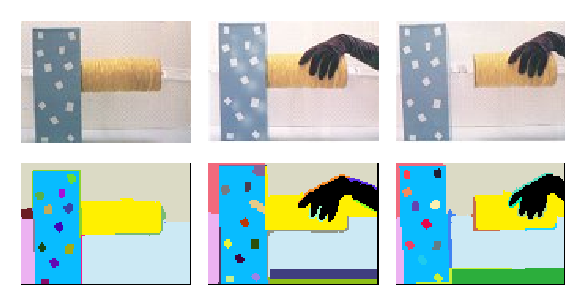
\includegraphics[width=0.5\columnwidth]{fig-pull}}

\caption{
Top: photos of one of Needhan's experiments; a yellow tube is 
pulled away from a blue box with white dots.
Bottom: segmentation of the photos.
}

\label{fig:move-apart}

\end{figure}

In this section we look at experiments that evaluate infant's
expectations about what should move together and what will move
independently; we will compare this to what is technically achievable.
For example, Figure~\ref{fig:move-apart} shows a scenario presented to
infants.



\begin{quote}

It is conceivable that young infants are not exposed to sufficient
contrastive evidence within the context of occlusion events. For
example, infants may seldom observe occlusion events in which: (a) the
objects seen to each side of an occluder either share, or do not
share, the same surface features; and (b) a judgment about the number
of objects present can only be made based on surface features. Without
such evidence, it would be difficult for infants to identify surface
features as important. Even once identified, infants may have few
opportunities to use, and to test, this new knowledge. If surface
features are indeed a less reliable source of information than form
features (e.g. see below), the opportunity to experiment with this new
knowledge might be necessary before infants would be disposed to use
it spontaneously. (Wilcox)

\end{quote}





\subsection{A technical evaluation of Gestalt principles}

How hard is spatiotemporal grouping?
Hard, in the general case.
Of a single, fixated object, while head is not moving much?  and
motion of head is available?

Still tough to do in real time, but the data is there in a form
we could process, given world enough and time.


Motion first -- then shape -- then color/pattern

What is there to learn about shape?  How to see it.

Needham 1999 result is not consistent with the direction of comp
vision research.  Algorithms would group two adjacent objects with
same color-and-pattern but different shapes long before grouping two
adjacent objects with same shape but different color-and-pattern.
Shape is inherently non-local, which color-and-pattern 
can at least to some extent be treated as a local feature.
Computationally, there 
has been little success in recovering shapes in cluttered static scenes.

Why could it make sense?  Lighting variation, color constancy is
really complicated -- maybe better to ignore until had a lot
of experience?

Appearance of surface is subject to a multiplicative effect
with its environment -- shadows, interreflections.

issue of 3D shape, 2D contours.

invariance versus selectivity, classic tradeoff.

If we start with motion, then what we have is motion silhouettes.
We can align the silhouette with the scene, and attempt to train
up methods for predicting the silhouette from the scene.
For a *particular* object at a particular time, it would seem 
best to use all the available correlated features, including 
surface features.  

Why would surface-info not be used in Needham1999 situation,
or be overridden by shape?

Suggest (1) train up generic boundary predictor, so
shape is perceivable, and (2) when shape is available,
segment based on it

Shape information is more important for actually doing things.

(could have more than silhouette from motion of course).


Shape in these particular experiments is maybe not that hard to
recover.

Maybe shape info is easier to use to link motion segmentation
events?  More trustworthy?  Cluster based on shape cues?

For my thesis, with a bunch of segmentations, clusturing by
some course shape measures gave around 88\% accuracy while
clustering by color histogram gave around 99\% accuracy.
But the robot was living in one corner of a lab, with 
relatively constant lighting.  In real life, the story may
be quite different.  Any evidence to suggest this?

Also, the development from grouping anything that moves
together, to then using gaps, is novel and interesting.
Get the cite.




\subsection{Possibilities}

``separately moving'' is not totally clear - consider e.g. a 
jacket, can move arms around a certain amount without body.

Bottom up or top down?  Bottom up and top down?  Interaction
with recognition?

Most commonly, but not always, segmentation is implemented
as a precursor to recognition.  Image comes in, gets
segmented, segments are then run through recognizer.

This is problematic, since segmentation without
recognition is relatively brittle -- it is uninformed.
For something like finding faces, it is more common
not to segment first -- but the common trick here
is to try all possible regions.

Good features, a progression.


\section{INTRO}


Johnson et al re segregation in the presence of partial occlusion.



\noindent General interests:

\begin{itemize}

\item Experiments that demonstrate ``development'' based on experience,
   particularly single or small numbers of episodes

\item Behaviors of the child/robot that have been demonstrated/argued
   to help generate good experience or otherwise help with development.

\end{itemize}


\subsection{Importance of motion?}

We are talking about the {\em development} of perception from an
immature form.  We assume that this development relies on acquiring
some information from the outside world (this isn't necessarily so).
How is this information acquired?  Sensory input is not 
uniformly difficult to interpret -- there are situations in
which it becomes simpler.  One particularly striking case is
the presence of motion.  Coherent group motion of part of the 
scene can be relatively easy to detect, and is a good cue for
the existence and extent of a corresponding object.  
So motion is one good place to start.
%
Moving objects are salient to infants and seem to play an
important role in perceptual learning (BACK THIS UP).
%
In robotics motion has frequently been used in all sorts of
ways.
%
Mention the technical status of motion detection versus
detection of other features (e.g. ``material'').
%
Of course this is by no means the end of the story, there 
are many other features... depth cues etc.

Egomotion is not very useful (relatively speaking).  Movemement of
others or caused by others is useful.  Motion caused by the robot
itself is particularly useful; this could be true of infants but is
moot given the limited motor control available initially.

\subsection{Preamble}

What is perception for?  One classic answer from robotics is that the
goal of perception is to recover, as faithfully as possible, the state
of the world.  That is, some model is made of the world, with some
number of free parameters, and the goal of perception is to find
values for those parameters to bring the model into as close an
alignment as possible with the world.

This view is my no means unquestioned; to achieve a particular
task, the most useful model to estimate may vary.  It may be
trivial, or the robot's behavior may be easier to produce or
describe in alternate ways that don't use the language of
model estimation.

In this paper, we will assume that the robot is engaged
in manipulation tasks (as opposed to, for example, navigation).

{\bf Behavioral view}: strategies that make it likely for the robot
to be looking somewhere useful (hand/eye coordination).
{\bf Model view}: ability to demonstrate flexible knowledge of presence of 
objects and some of their properties.


\subsection{Formalities}

Should provide the clearest possible definition of terms,
as a reference.  Human and robot uses of terms could deviate
from this definition if the deviation is also clearly described.

Object segregation, intermodal integration, object permanence.

Define a cell as the smallest sensing unit, for whichever sensors are
under consideration (e.g. pixels for images).  Assume there are a
fixed number of cells $c_1...c_{N}$.

There is also an unknown set of causes $s_1...s_{M}$, which for a
bounded period of consideration we will consider fixed.  Each cell
$c_i$ provides varying sensor readings $c_i(t)$.  We would like to
generate assignments $a_j(t)$ which, for each cause, lists all the
cells that can reasonably be attributed to that cause.  Then we choose
our causes to be maximally useful in describing the environment.

It is a little difficult to say exactly what judgement should be
made in complicated cases.  Might be better to give examples,
and underspecify.

Specification for object segregation:

$I(t) = [c_1.val(t) ... c_N.val(t)]$

Goal of segregation:
  Find a set $S_i$ = e.g. ${ c_2,c_4,c_5,c_6,... }$ that lists cells that
  belong together at a particular time.
  Find a set of such sets - Z.

Goal of intermodal integration:
  Bring together such sets across modal boundaries.

Goal of object permanence:
  Bring together such sets across time and disappearances.


***********

stuff to be integrated [from Lorenzo]:


The paper focuses on objects. Can we say something about the role of the
body? Achieving eye-hand coordination proved to be extremely useful on the
robots we have worked on. Learning to act is necessary to perform active
exploration of objects (poking/pushing/tapping/grasping). During action the
ability to identify the body helps the robot to focus the attention on the
area of the visual space where "things are happening" (i.e. on the hand upon
contact with the object).


***********

Big potential difference between infants and humans: the role
of manipulation in shaping early perception.  Infants can't
act that much to begin with.



